\section{Istruzione per l'utilizzo}
  L'header della {dashboard}\ped{G} è uguale come struttura per ogni tipo di utente. Su di esso troviamo un link che porta alla modifica dei dati personali, chiamato \textit{Profilo}, e un link, \textit{Esci}, che, se cliccato, effettua il logout dal sistema.



\subsection{Interfaccia}
    \begin{figure}[H]
        \centering
   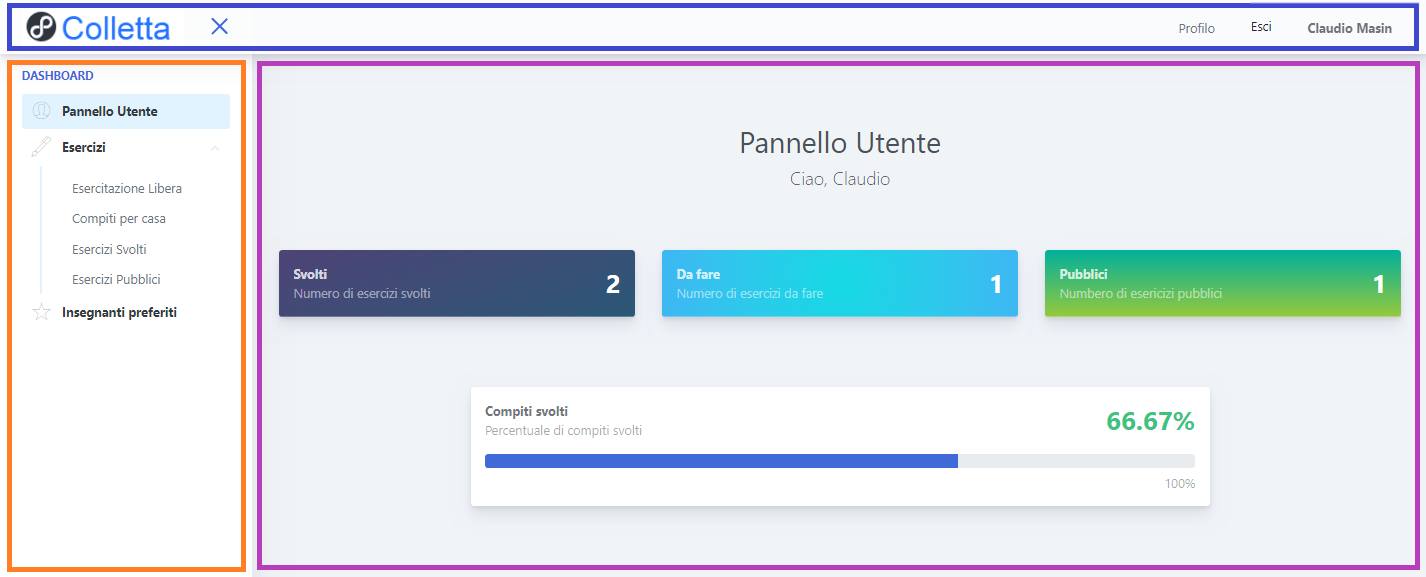
\includegraphics[width=17cm]{sez/img/istruzioni/panoramica.png} 
        \caption{Panoramica dell'interfaccia}\label{fig:1}
    \end{figure}
  La struttura generale di una pagina è la stessa per ogni utente loggato. Sono presenti i seguenti elementi di base:
    \begin{itemize}
        \item Barra del menu;
        \item {Sidebar}\ped{G};
        \item Contenuto della pagina.
    \end{itemize}
 A seconda del tipo di utente (Allievo, Insegnante, Sviluppatore, Amministratore) e della pagina selezionata, verranno visualizzati a schermo contenuti diversi. Ogni utente ha comunque a disposizione lo stesso header e un link al suo pannello utente.


\subsection{Utente non autenticato}
    \subsubsection{Registrazione}
    	\begin{figure}[H]
        	\centering
        	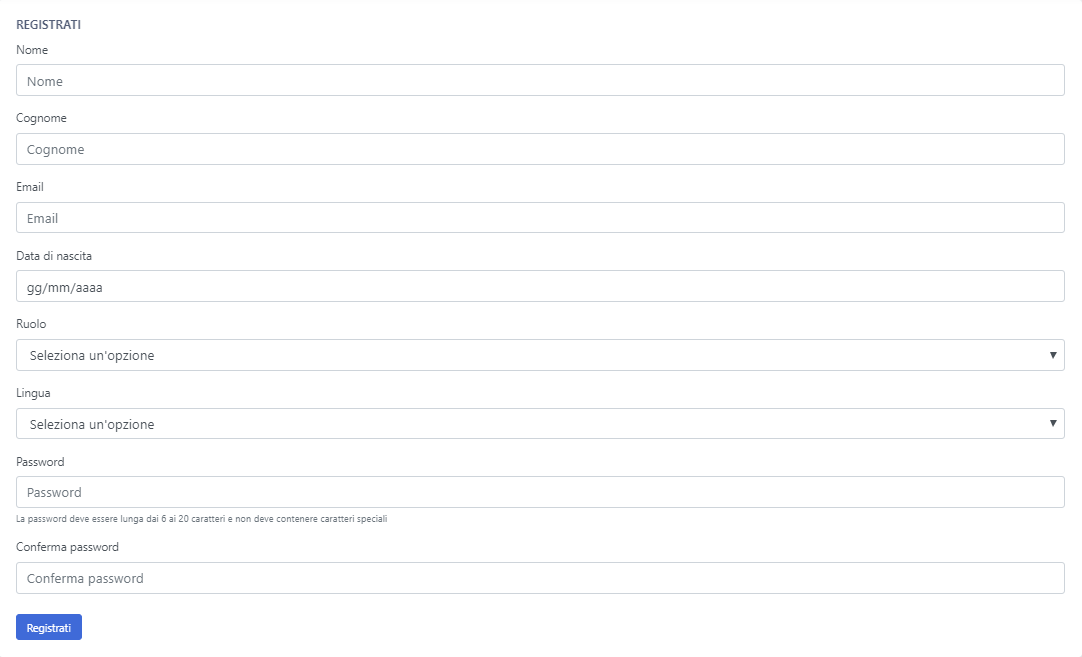
\includegraphics[width=1\linewidth]{sez/img/autenticazione/formRegistrazione.PNG} 
        	\caption{Registrazione utente}\label{fig:registrazione}
    	\end{figure}
	   Se non si è ancora registrati è possibile farlo cliccando sul bottone \textit{Registrati} presente nella barra del menu. Una volta compilato il {form}\ped{G} viene inviata una mail per l'attivazione dell'account. E' necessario cliccare sul link appena ricevuto, successivamente verrà aperta una pagina con un messaggio di conferma. A questo punto se il ruolo scelto è \textit{Insegnante} o \textit{Allievo} è possibile accedere alla piattaforma; se \textit{Sviluppatore} è necessario attendere anche l'attivazione manuale da parte di un  \textit{Amministratore} della piattaforma. I dati sono tutti obbligatori e il form visualizzato è quello in \autoref{fig:registrazione}.
    \subsubsection{{Login}\ped{G}}
    	\begin{figure}[H]
        	\centering
        	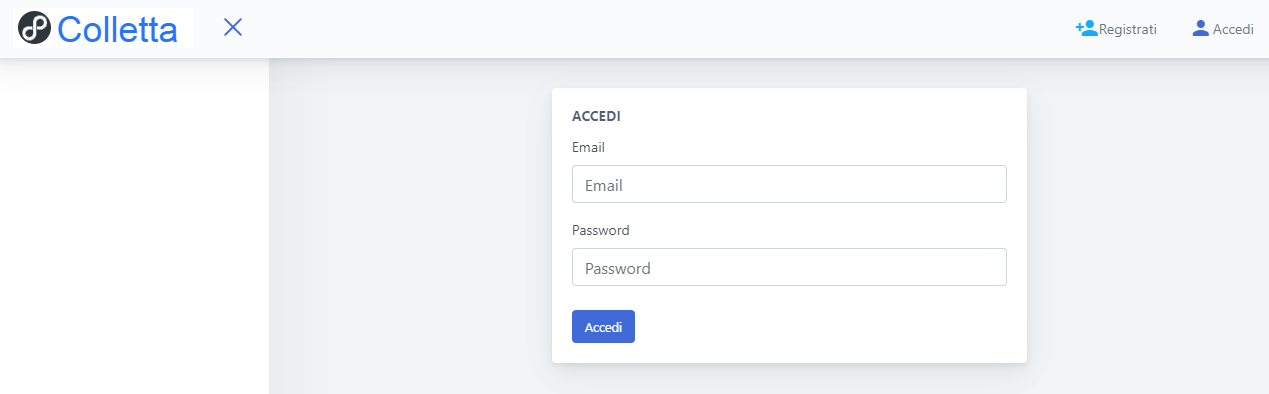
\includegraphics[width=1\linewidth]{sez/img/autenticazione/formAccedi.PNG} 
        	\caption{Inserimento credenziali per l'accesso}\label{fig:1}
    	\end{figure}
Una volta effettuata la registrazione, per poter accedere alla piattaforma è necessario recarsi sull'apposita pagina collegata dal link in altro a destra \textit{Accedi}, inserire l'email, la propria password e successivamente cliccare sul pulsante \textit{Accedi} del form.

    \subsubsection{Password dimenticata}
    	\begin{figure}[H]
        	\centering
        	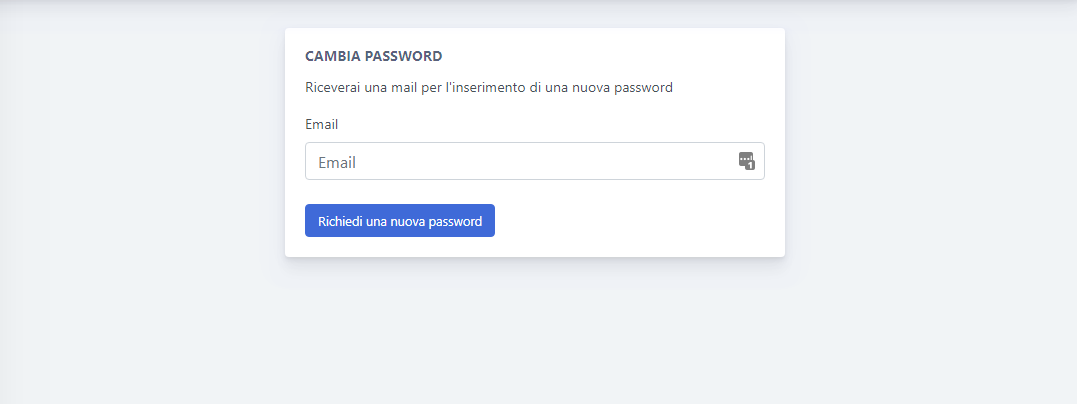
\includegraphics[width=1\linewidth]{sez/img/autenticazione/passwordDimenticata.png} 
        	\caption{Conferma email per il recupero della password}\label{fig:1}
    	\end{figure}
	L'unico modo per cambiare la password di un utente iscritto alla piattaforma è  tramite il form di recupero password. Cliccando sul link \textit{Password dimenticata?} presente all'interno del form di login, compare un form con una casella di testo per l'inserimento della mail utilizzata durante la registrazione. 
	
	Cliccando il pulsante \textit{Richiedi una nuova password}, se esiste effettivamente un account collegato a 	quella mail, viene inviata una mail contenente un link per l'inserimento della nuova password. Cliccandolo verrà aperta una pagina della piattaforma \textit{Colletta} con un form contenente due caselle di testo per l'inserimento della nuova password.
	
\begin{figure}[H]
        	\centering
        	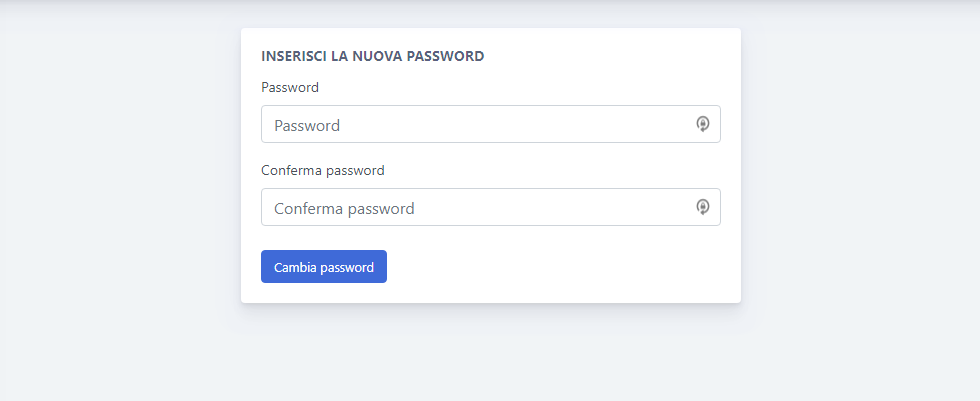
\includegraphics[width=1\linewidth]{sez/img/autenticazione/password.png} 
        	\caption{L'inserimento della nuova password}\label{fig:1}
    	\end{figure}	

Una volta inserita la nuova password è sufficiente cliccare il pulsante \textit{Cambia password}. Un messaggio di conferma indica che l'operazione è andata a buon fine.	
	
% UTENTE AUTENTICATO
\subsection{Utente autenticato generico}

    \subsubsection{Logout}
    Per effettuare il {logout}\ped{G} si deve cliccare sulla voce \textit{Esci} dalla barra del menu. Facendo ciò, l'utente termina la propria sessione.
    \subsubsection{Modifica dati}
    	\begin{figure}[H]
        	\centering
        	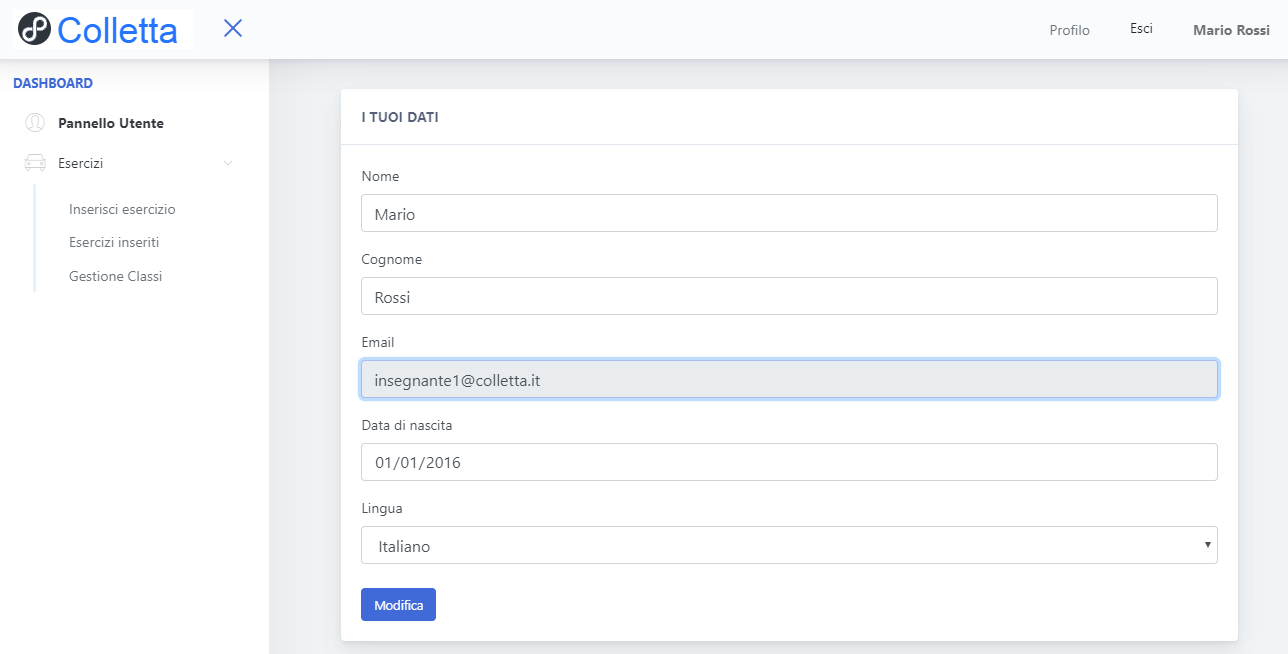
\includegraphics[width=1\linewidth]{sez/img/autenticazione/modati.PNG} 
        	\caption{Modifica dati personali}\label{fig:1}
    	\end{figure}
    Dopo aver effettuato la registrazione si accede cliccando su \textit{Accedi} nella barra del menu. E' necessario inserire email e password e successivamente cliccare sul pulsante \textit{Accedi} del form. La modifica dei dati è disponibile a ogni tipologia di utente.

\newpage
    \subsection{Allievo}
      L'allievo si iscrive nel portale \textbf{Colletta} per svolgere esercizi di analisi grammaticale. Può svolgere esercizi assegnati da un'insegnante o svolgere esercizi liberi tramite il sistema di correzione automatica del sistema. Esso ha la possibilità di confrontare la sua soluzione con quella presentata dal sistema ricevendo anche un voto.
      \\La sidebar dell'allievo presenta le seguenti voci:
            \begin{itemize}
                \item Pannello utente;
                \item Esercitazione libera;
                \item Compiti per casa;
                \item Esercizi svolti;
                \item Esercizi pubblici;
                \item Insegnanti preferiti.
            \end{itemize}
            

            
        \subsubsection{Pannello utente}
			\begin{figure}[H]
        		\centering
        		\includegraphics[width=1\linewidth]{sez/img/studente/panelloUtente.PNG} 
        		\caption{Panello utente: Allievo}\label{fig:1}
    		\end{figure}        
        
          Il pannello utente è un riassunto di tutti i progressi e le attività svolte dall'allievo. Il pannello utente mostra un messaggio di benvenuto,il numero di esercizi assegnanti, i suoi progressi, quanti esercizi ha svolto e quanti esercizi pubblici sono disponibili. 
          
		 \subsubsection{Esercitazione libera}      
        	\begin{figure}[H]
                \centering
                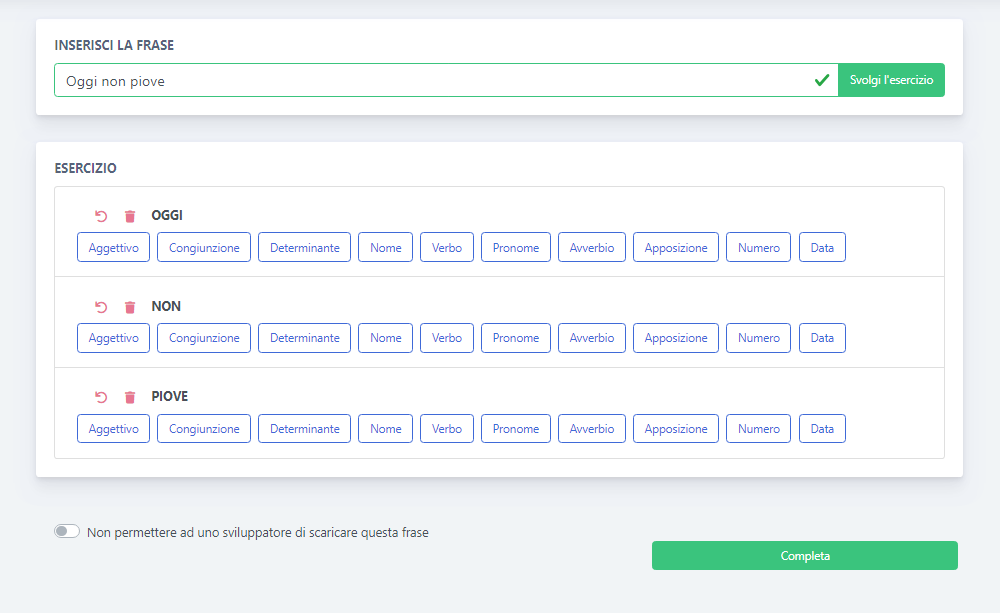
\includegraphics[width=17cm]{sez/img/studente/esercitazioneLiberaEsegui.PNG} 
                \caption{Svolgimento esercizio libero}\label{fig:1}
        	\end{figure}
          In questa pagina è possibile svolgere un esercizio inserendo nella casella di testo una frase da analizzare. La soluzione appena inserita viene confrontata con quella generata automaticamente.
        \\ Svolgimento:
        	\begin{enumerate}        
            	\item Scrivere la frase da analizzare all'interno della casella di testo;
            	\item Cliccare su \textit{Svolgi l'esercizio};
            	\item Svolgere l'esercizio e cliccare \textit{Completa}.
        	\end{enumerate}
        	\label{sec:esLib}
        	Lo svolgimento dell'esercizio è guidato, ogni pulsante rappresenta una scelta possibile, il primo pulsante selezionato corrisponde alla categorica alla quale appartiene la parola, le scelte successive raffinano l'analisi. Ad ogni click di un pulsante vengono generati dei pulsanti strettamente collegati a quello precedente. In caso non comparissero più pulsanti, significa che l'analisi per quella parola è terminata. In ogni momento l'allievo può decidere di resettare la soluzione per una determinata parola (icona cestino), o annullare l'ultima scelta (freccia indietro).        \linebreak	
        A sinistra del pulsante completa è presente un {flag}\ped{G} che indica se la frase appena inserita può essere messa a disposizione degli sviluppatori che utilizzano i dati della piattaforma, non selezionandolo si acconsente la condivisione di questo dato.
        	

        \newpage
  		\subsubsection{Compiti per casa}
 		  In questa sezione l'allievo ha la possibilità di visualizzare gli esercizi a lui assegnati e sceglierne uno da svolgere.
        	\begin{figure}[H]
            	\centering
            	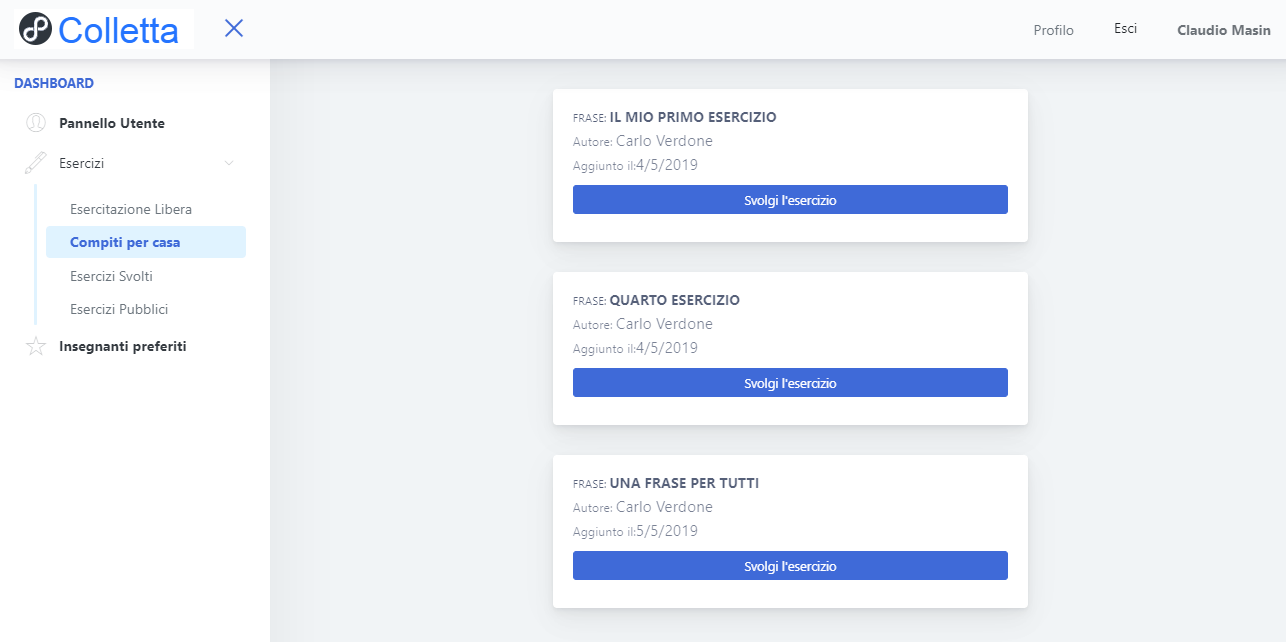
\includegraphics[width=17cm]{sez/img/studente/compitopercasa.PNG} 
            	\caption{Scelta esercizio da svolgere}\label{fig:1}
        	\end{figure}

		  E' possibile scegliere l'esercizio da svolgere cliccando sul pulsante \textit{Svolgi l'esercizio}. 
		  
		  
		    \paragraph{Svolgimento esercizio scelto}\mbox{}\\
		    Una volta selezionato l'esercizio di apre una pagina per lo svolgimento, contenente un set di scelte per ogni parola appartenente alla frase dell'esercizio.     
       
        	\begin{figure}[H]
            	\centering
            	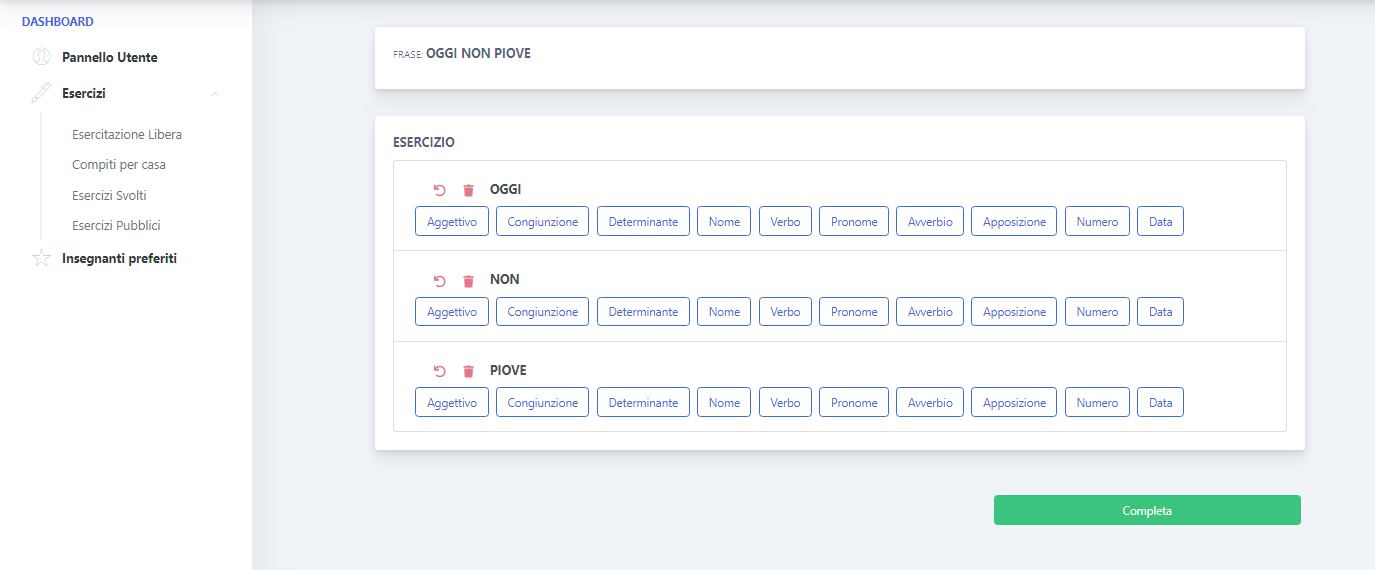
\includegraphics[width=17cm]{sez/img/studente/svolgimentoesercizio.PNG} 
            	\caption{Svolgimento esercizio}\label{fig:1}
        	\end{figure}      
	L'allievo esegue quindi l'analisi della frase allo stesso modo descritto in \S\ref{sec:esLib}. La soluzione visualizzata alla fine sarà in questo caso quella dell'insegnante che ha assegnato l'esercizio. 
	
	\begin{figure}[H]
            	\centering
            	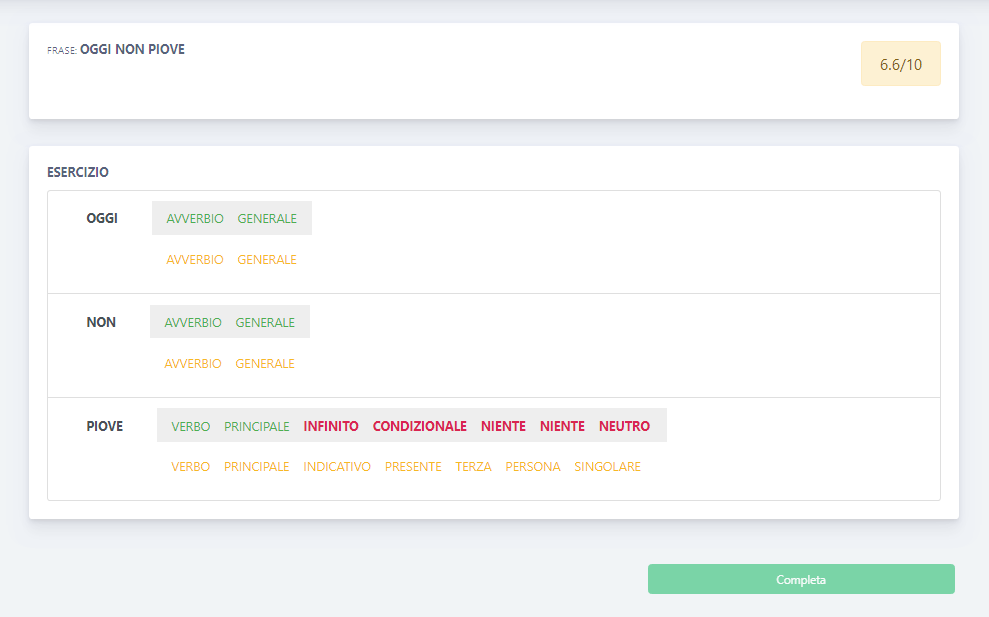
\includegraphics[width=17cm]{sez/img/studente/risultatoEsercizio.png} 
            	\caption{Risultato esercizio svolto}\label{fig:1}
        	\end{figure}     
        Le scelte uguali a quelle della soluzione dell'insegnante vengono evidenziate in verde mentre quelle diverse in rosso. In alto a destra viene mostrato il voto in decimi calcolato automaticamente paragonando la soluzione con quella dell'insegnante.
        
        \subsubsection{Esercizi svolti}
        	\begin{figure}[H]
            	\centering
            	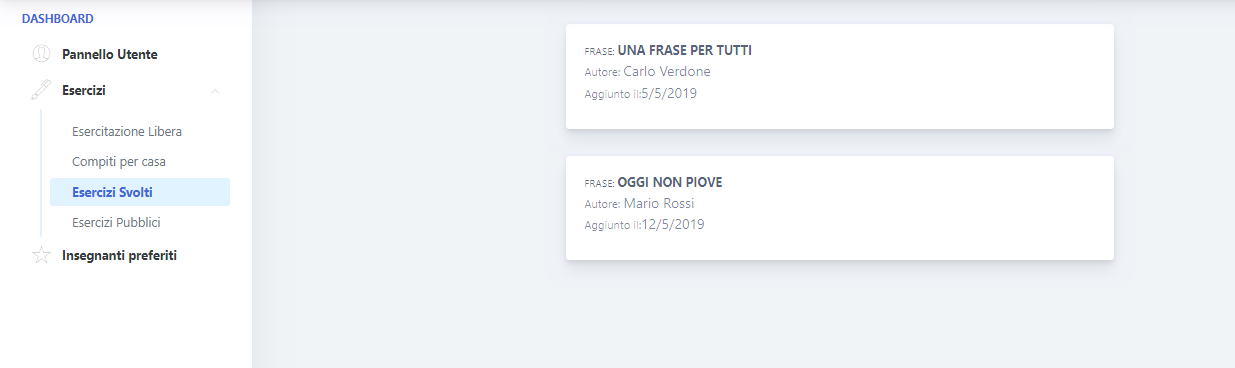
\includegraphics[width=17cm]{sez/img/studente/esercizisvolti.PNG} 
            	\caption{Storico esercizi svolti}\label{fig:1}
        	\end{figure}
          In questa pagina è possibile visualizzare lo storico degli esercizi che sono stati svolti. Per ogni esercizio svolto sono visualizzabili la data di aggiunta, la frase analizzata e il nome dell'insegnante che ha assegnato l'esercizio.
          
          
           \subsubsection{Esercizi pubblici}
        	\begin{figure}[H]
            	\centering
            	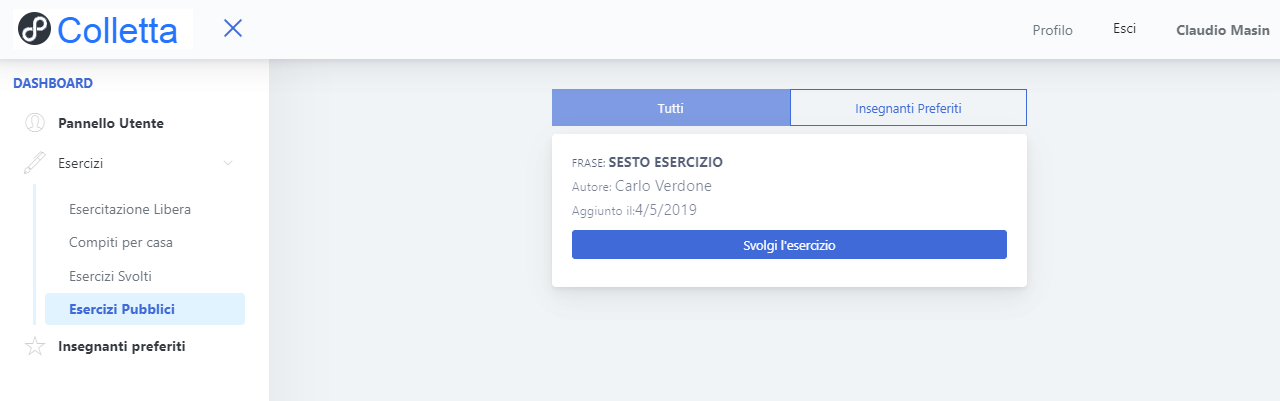
\includegraphics[width=17cm]{sez/img/studente/esercizipubblici.PNG} 
            	\caption{Elenco esercizi pubblici}\label{fig:1}
        	\end{figure}
        	In questa pagina è possibile visualizzare tutti gli esercizi resi pubblici dagli insegnanti. Si ha abbiamo la possibilità  di scegliere tra gli esercizi inseriti da un qualsiasi insegnante oppure solo tra quelli aggiunti tra gli insegnanti preferiti. Possiamo quindi svolgerli come un normale esercizio. 
        
        
        
\subsubsection{Insegnanti preferiti}
        	\begin{figure}[H]
            	\centering
            	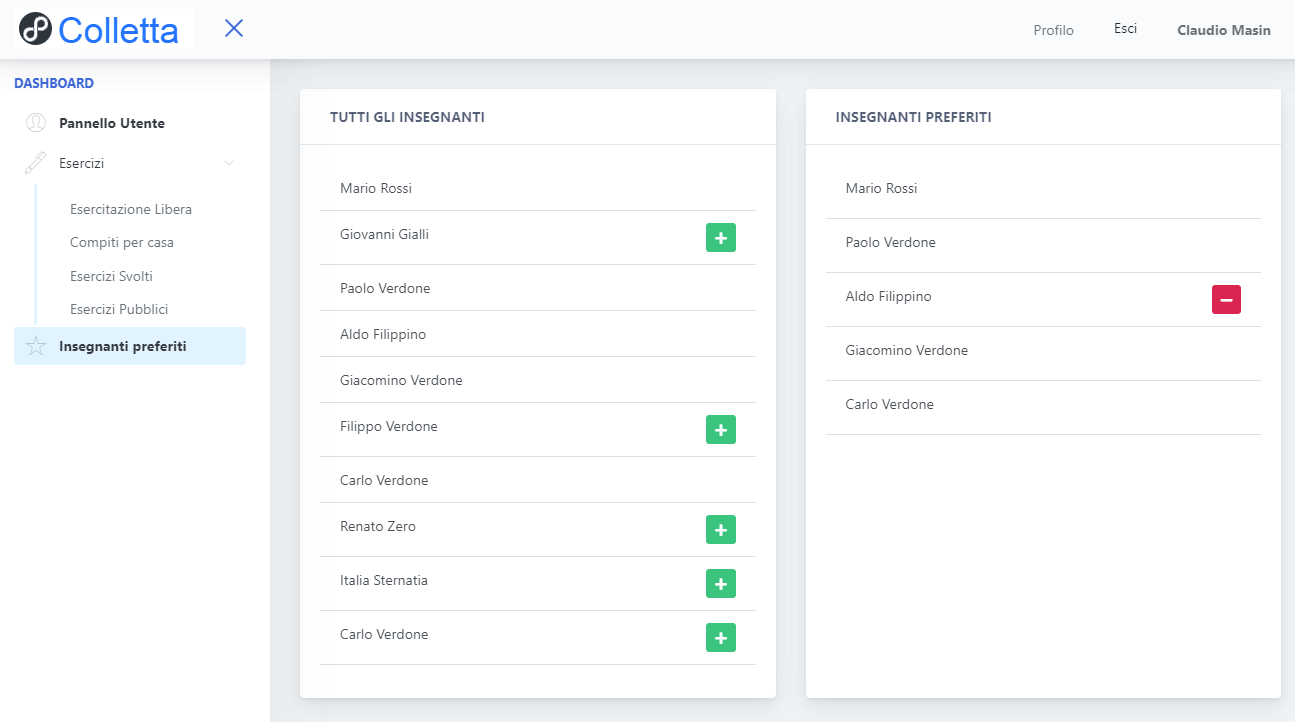
\includegraphics[width=17cm]{sez/img/studente/insegnantepreferito.png} 
            	\caption{Elenco insegnanti preferiti}\label{fig:1}
        	\end{figure}        
        In questa pagina troviamo l'elenco di tutti gli insegnanti presenti nella lista di sinistra cliccando sul pulsante \textit{"+"} possiamo aggiungerli tra gli insegnanti preferiti, se invece si vuole rimuovere un insegnante dalla lista è sufficiente cliccare sul pulsante \textit{"-"} che compare se il cursore viene avvicinato al nome dell'insegnante che si vuole rimuovere.
        
        
        
\newpage
    \subsection{Insegnante}
      L'insegnante è l'utente che può inserire esercizi privati o decidere di assegnarli ai propri allievi. 
         \\La sidebar dell'insegnante presenta le seguenti voci:
        	\begin{itemize}
            	\item Pannello utente;
            	\item Inserisci esercizio;
            	\item Esercizi inseriti;
            	\item Gestione classi.
        	\end{itemize}
        
        
        
        \subsubsection{Pannello utente}
        \begin{figure}[H]
        		\centering
        		\includegraphics[width=1\linewidth]{sez/img/insegnante/panelloUtente.PNG} 
        		\caption{Panello utente: Insegnante}\label{fig:1}
    		\end{figure}
          Il pannello utente mostra un messaggio di benvenuto all'insegnante, un riepilogo con il numero di esercizi inseriti, le classi create e gli studenti presenti nel sistema.
        
        \newpage
        \subsubsection{Inserisci esercizio}
          La funzione principale dell'insegnante è quello di inserire esercizi all'interno del sistema ed assegnarli agli alunni.
        	\begin{figure}[H]
            	\centering
        		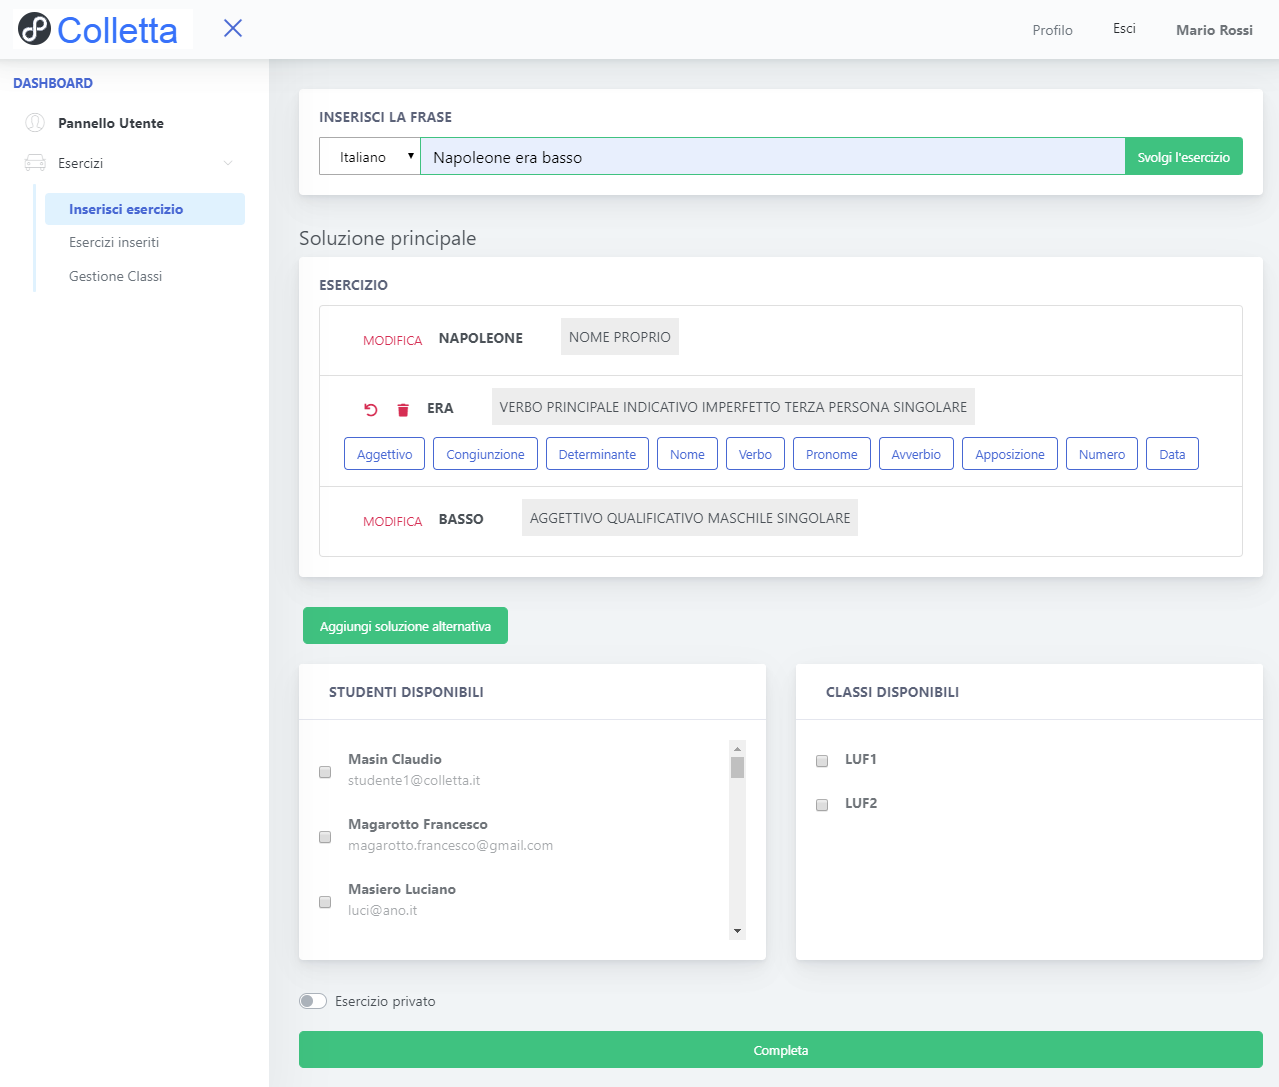
\includegraphics[width=17cm]{sez/img/insegnante/inserisciEsercizio.PNG} 
            	\caption{Inserimento e assegnazione esercizio}\label{fig:1}
        	\end{figure}
        
         
          Dopo aver inserito la frase, verrà visualizzata la correzione automatica. Se è ritenuto necessario è possibile modificare la soluzione cliccando sul pulsante \textit{Modifica}; se cliccato, viene eliminata la soluzione proposta dal sistema per quella parola e chiesto di inserire una nuova soluzione. 
          
          Durante l'inserimento manuale della soluzione l'insegnante ha la possibilità di tornare indietro di un passo o di resettare completamente la soluzione appena inserita. Questo processo è analogo a quello presentato in \S\ref{sec:esLib}. 
          Se è necessario, è possibile inserire una soluzione alternativa; cliccando sul pulsante \textit{Aggiungi soluzione alternativa} si apre un box identico a quello della soluzione principale; la modalità dell'inserimento della soluzione infatti è la stessa della soluzione principale. 
          
           Finita la correzione, l'insegnate può assegnare l'esercizio a un allievo selezionandolo dalla lista a sinistra sotto le soluzioni inserite oppure può assegnarlo direttamente ad una classe di studenti precedentemente creata selezionandola dall'elenco a destra sotto le soluzioni. 
          
          Prima di completare l'inserimento dell'esercizio, a sinistra abbiamo due flag grazie a loro, si può scegliere se rendere l'esercizio privato in modo che non venga aggiunto  nella lista degli esercizi pubblici e impedire agli sviluppatori che utilizzano i dati raccolti dalla piattaforma di scaricare anche quest'ultimo. 
          
            Cliccando sul pulsante \textit{Completa} l'esercizio viene aggiunto al sistema.
          
\subsubsection{Esercizi inseriti}
\begin{figure}[H]
            	\centering
        		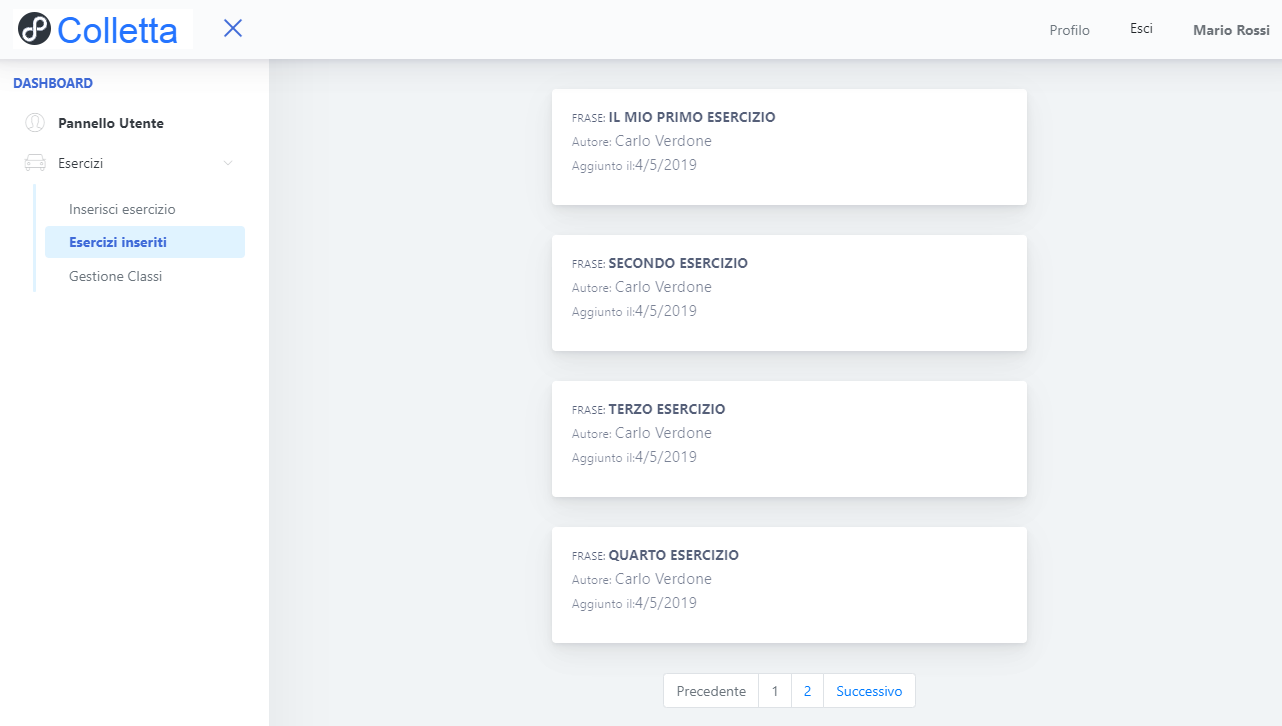
\includegraphics[width=17cm]{sez/img/insegnante/eserinseriti.PNG} 
            	\caption{Elenco esercizi svolti}\label{fig:1}
        	\end{figure}  
        	In questa pagina è presente l'elenco di tutti gli esercizi inseriti dal insegnante. Gli esercizi sono impaginati a gruppi di quattro.
        	
        	 Cliccando sopra un esercizio è possibile visualizzare i suoi dettagli.               
\newpage
\paragraph{Dettagli esercizio}\mbox{}\\   

\begin{figure}[H]
            	\centering
        		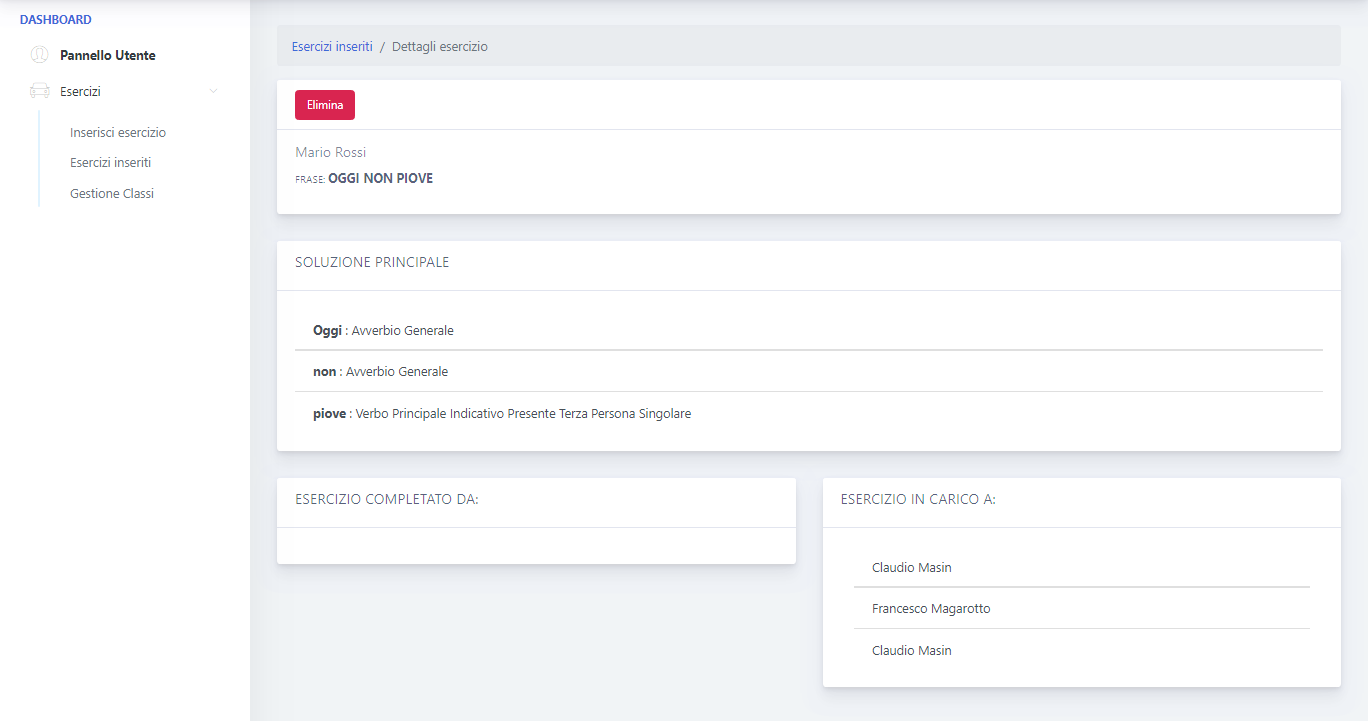
\includegraphics[width=17cm]{sez/img/insegnante/detagliesercizio.PNG} 
            	\caption{Tutti i dettagli di un esercizio}\label{fig:1}
        	\end{figure}     	
        	In questa pagina è presente il testo dell'esercizio, eventuali soluzioni, la lista degli alunni che hanno completato l'esercizio e la lista degli alunni che lo devono ancora svolgere.
        	
        	
        	Cliccando sul pulsante \textit{Elimina} è possibile eliminare completamente l'esercizio dal sistema, rimuovendolo automaticamente anche dalla lista dei \textit{Compiti per casa} dei vari allievi.
        	
\newpage
        \subsubsection{Gestione classi}   
       
        \begin{figure}[H]
            	\centering
        		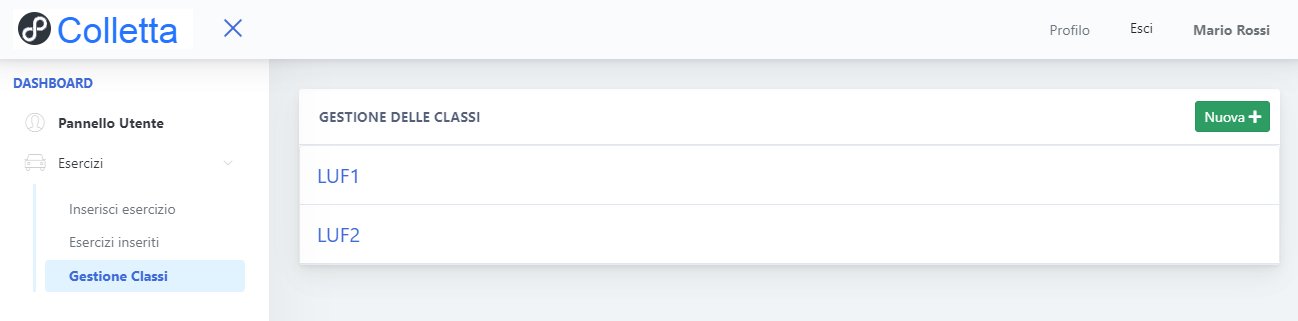
\includegraphics[width=17cm]{sez/img/insegnante/elencoclassi.PNG} 
            	\caption{Gestione delle classi}\label{fig:1}
        	\end{figure}          	
        	   
        In questa pagina è possibile creare, eliminare e modificare classi di allievi. 

\paragraph{Creazione nuova classe}\mbox{}\\         

\begin{figure}[H]
            	\centering
        		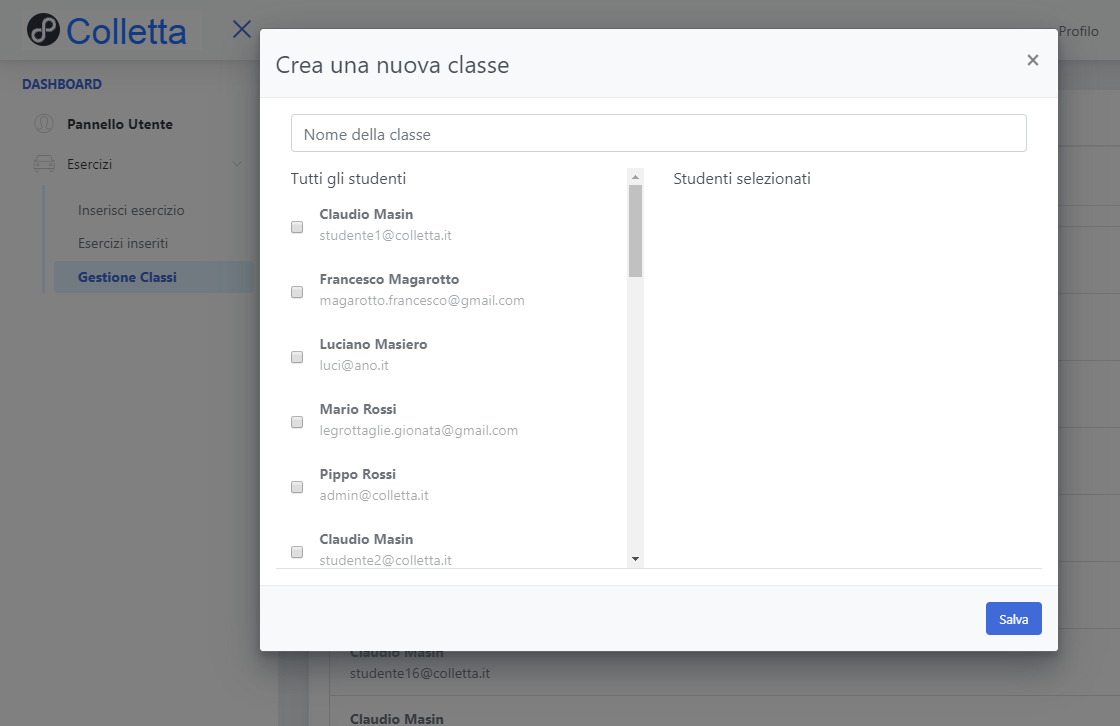
\includegraphics[width=17cm]{sez/img/insegnante/creanuovaclasse.PNG} 
            	\caption{Creazione nuova classe}\label{fig:1}
        	\end{figure}            	

Cliccando sul pulsante  \textit{Nuova} compare una finestra sulla pagina. All'interno della casella di testo va inserito il nome che si vuole attribuire alla nuova classe; per aggiungere gli allievi è sufficiente selezionarli dalla lista sottostante. Gli allievi selezionati compaiono anche nella lista alla destra per rendere più chiaro il risultato finale ottenuto. 

Cliccando sul pulsante \textit{Salva} la classe viene salvata nel sistema. D'ora in avanti è possibile utilizzarla durante l'inserimento di nuovi esercizi.
 
 \paragraph{Gestione classe}\mbox{}\\
 
 \begin{figure}[H]
            	\centering
        		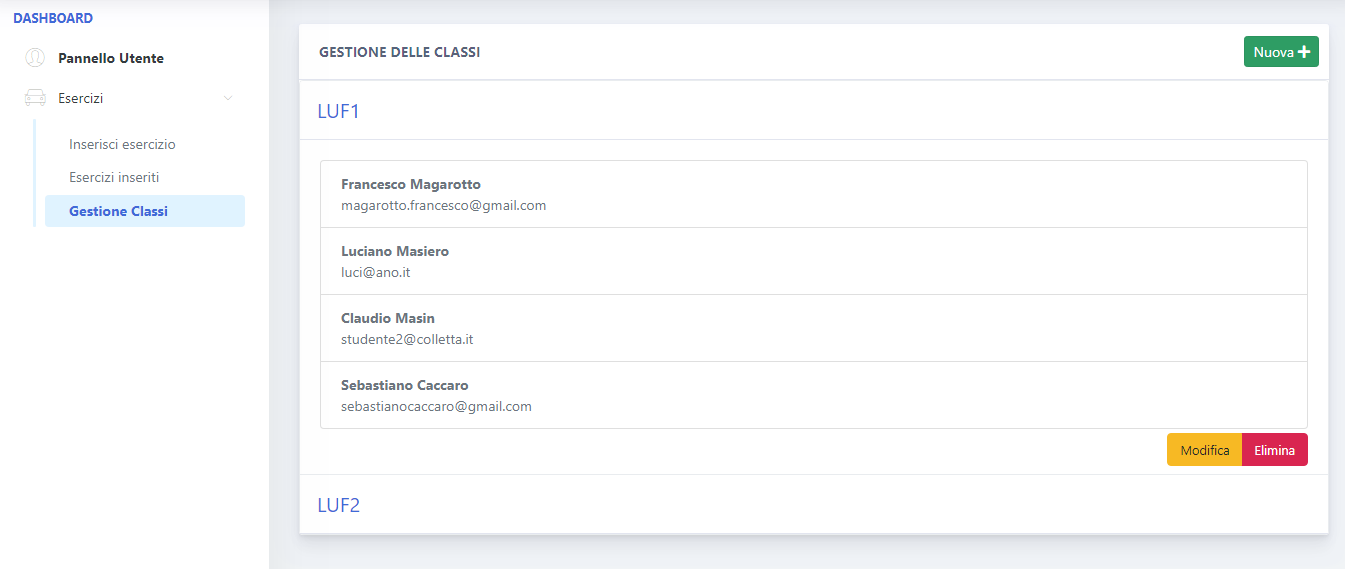
\includegraphics[width=17cm]{sez/img/insegnante/gestioneclasse.PNG} 
            	\caption{Detagli di una classe}\label{fig:1}
        	\end{figure}
        	
 Cliccando su una singola classe si espande un pannello contenente la lista degli allievi precedentemente aggiunti.
Una volta aperto il pannello è possibile eliminare o modificare una classe.
Cliccando il pulsante \textit{Elimina} compare un box che richiede la conferma per effettuare l'operazione, cliccando \textit{SI} la classe viene eliminata, cliccando \textit{NO} l'operazione viene annullata.
 \begin{figure}[H]
            	\centering
        		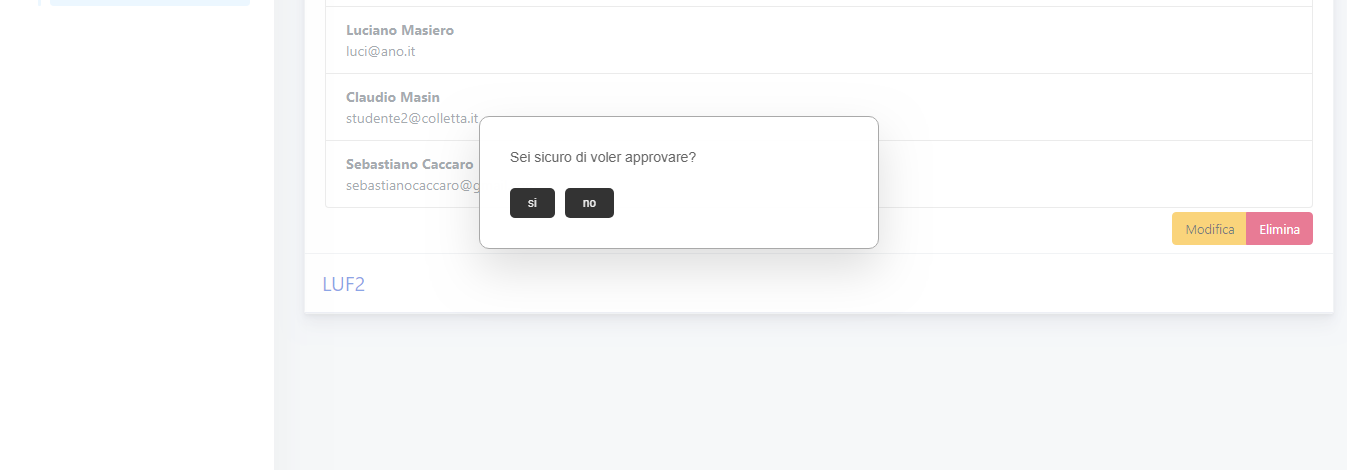
\includegraphics[width=17cm]{sez/img/insegnante/confermaElimina.png} 
            	\caption{Conferma eliminazione}\label{fig:1}
        	\end{figure}
     
       
       \newpage
         \paragraph{Modifica classe}\mbox{}\\	      
        
         \begin{figure}[H]
            	\centering
        		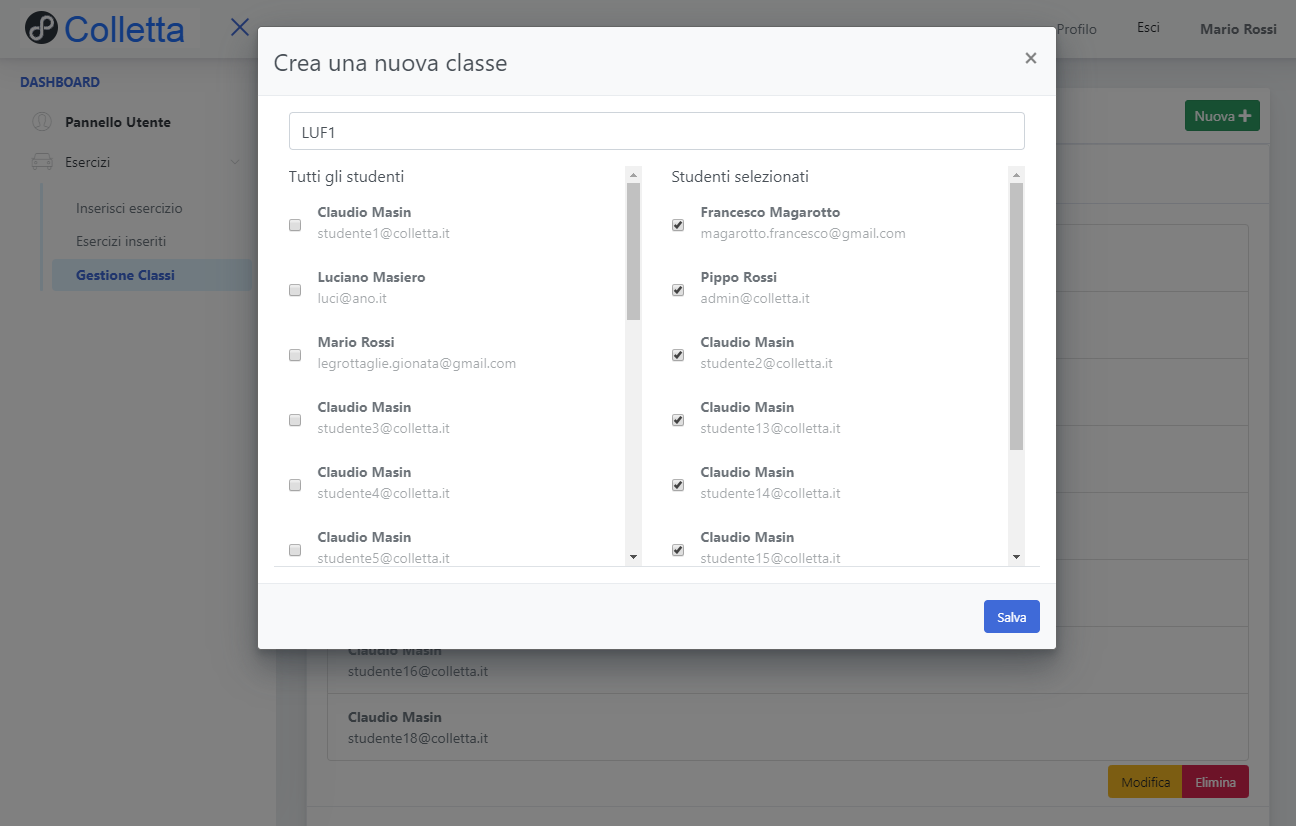
\includegraphics[width=17cm]{sez/img/insegnante/modificaclasse.PNG} 
            	\caption{Modifica una classe}\label{fig:1}
        	\end{figure}
        	
        	
Cliccando su \textit{Modifica} compare la finestra che ci permette di aggiungere nuovi allievi, rimuoverli o eventualmente modificare il nome. Per salvare le modifiche è sufficiente cliccare sul pulsante \textit{Salva}.
        
	\newpage
    \subsection{Sviluppatore}
    Lo sviluppatore compre un ruolo fondamentale all'interno della piattaforma. Egli è colui che utilizzerà i dati inseriti da \textit{Allievi} e \textit{Insegnanti}, con l'obiettivo di utilizzarli come input per i sistemi di autoapprendimento.
    Lo sviluppatore può iscriversi alla piattaforma utilizzando lo stesso sistema utilizzato dagli altri tipi di utenti a differenza dell'attivazione dell'account. E' necessario l'attivazione manuale da parte di un amministratore della piattaforma per poter accedere la prima volta. 
        	 \\Il pannello utente è l'unica pagina presente all'interno dell'area riservata di uno \textit{Sviluppatore}.
   
    	\subsubsection{Pannello utente}
    				\begin{figure}[H]
				\centering
				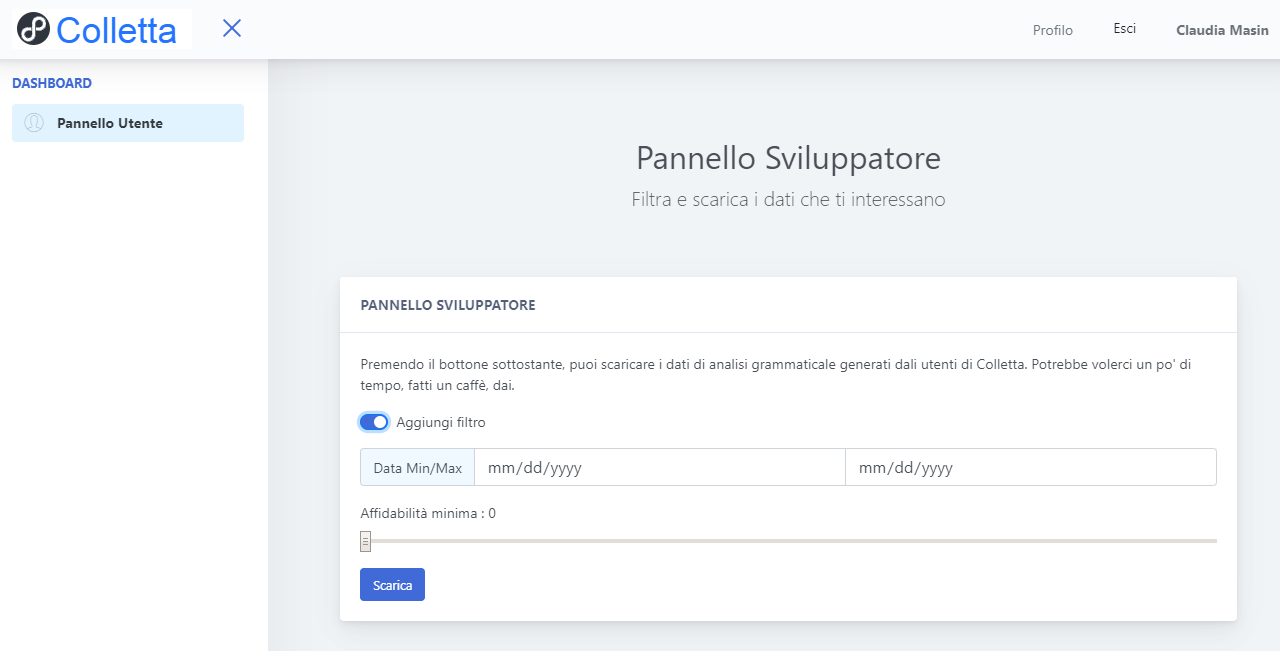
\includegraphics[width=17cm]{sez/img/sviluppatore/panelloutente.PNG}
				\caption{Pannello utente: Sviluppatore}\label{fig:1}
			\end{figure}
			 All'interno del pannello è presente un pulsante per scaricare tutti i dati presenti all'interno del sistema; eventualmente è possibile inserire dei filtri per avere dei dati che si avvicinano maggiormente alla proprie esigenze.
    	  Il pannello utente mostra un messaggio di benvenuto allo sviluppatore, che è libero di procedere allo scaricamento dei dati prodotti dagli utenti.
    	 Cliccando il flag \textit{Aggiungi filtro} compare un form contenente due caselle di testo per inserire un range di date in cui è stato inserito un esercizio e sotto di esso una barra di valori tra \textit{0 - 100} indicare l'affidabilità minima richiesta per una soluzione.
    	 Cliccando il pulsante \textit{Scarica} un file di formato {JSON}\ped{G} viene salvato all'interno della propria cartella predefinita dei download.

	\newpage
	\subsection{Amministratore}
	L'amministratore ha la possibilità di gestire tutti gli utenti che non siano amministratori, inoltre può approvare o declinare le richieste di iscrizione degli sviluppatori.
		  \\Voci nella sidebar:
			\begin{itemize}
				\item Pannello utente;
				\item Sviluppatori;
				\item Utenti.
			\end{itemize}



		\subsubsection{Pannello utente}
			\begin{figure}[H]
				\centering
				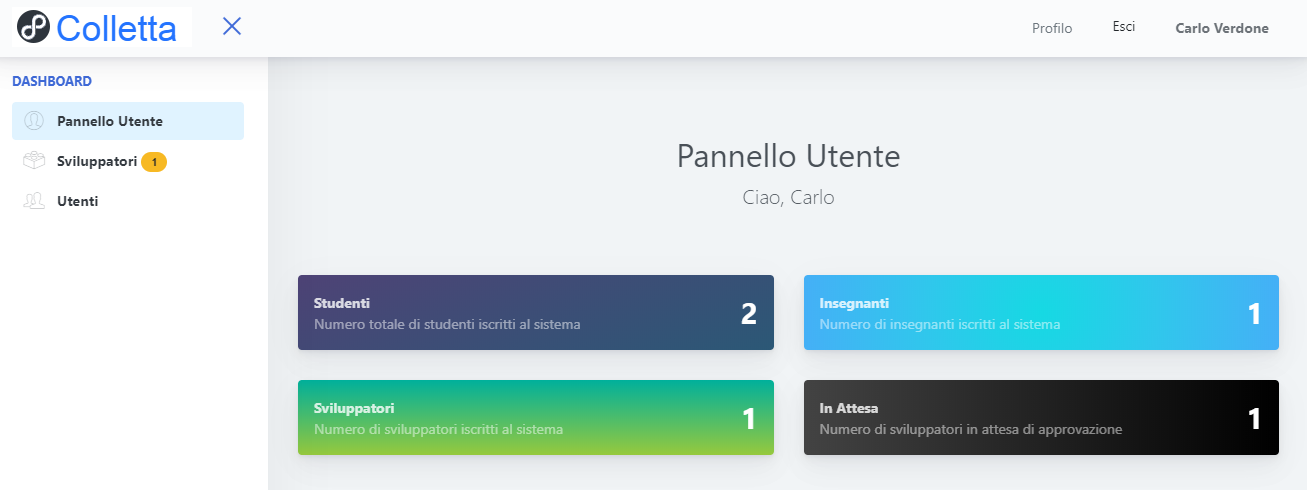
\includegraphics[width=17cm]{sez/img/amministratore/panelloadmin.PNG}
				\caption{Pannello utente: Amministratore}\label{fig:1}
			\end{figure}
		Il pannello utente contiene un breve riepilogo della situazione attuale all'interno della piattaforma.
		Sono presenti quattro box che indicano rispettivamente: il numero di \textit{Allievi} iscritti, il numero di \textit{Insegnanti} iscritti, il numero di \textit{Sviluppatori} iscritti ed approvati e il numero di \textit{Sviluppatori} iscritti ma ancora in attesa di approvazione.

		\subsubsection{Sviluppatori}
			\begin{figure}[H]
				\centering
				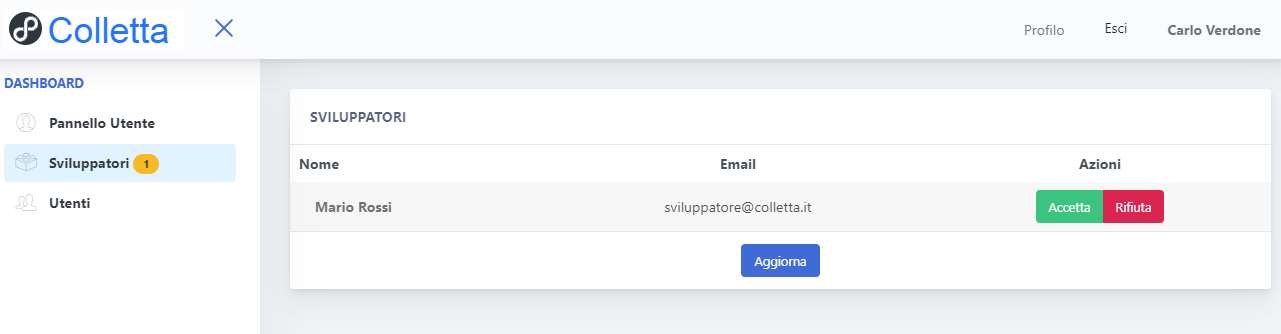
\includegraphics[width=17cm]{sez/img/amministratore/conf_ric_svil.PNG}
				\caption{Richieste di iscrizione degli sviluppatori}\label{fig:1}
			\end{figure}
		  In questa pagina l'amministratore può approvare o rifiutare le richieste di iscrizione degli sviluppatori. Viene presentata una lista contente gli sviluppatori che hanno richiesto di iscriversi al sistema. Ogni sviluppatore ha un nome e una mail. L'amministratore, premendo su \textit{Accetta}, consente allo sviluppatore di effettuare il login, premendo su \textit{Rifiuta} invece, rifiuta e cancella lo sviluppatore dal sistema. Premendo sul pulsante \textit{Aggiorna} viene ricaricata la lista degli \textit{Sviluppatori}.


		\subsubsection{Utenti}
			\begin{figure}[H]
				\centering
				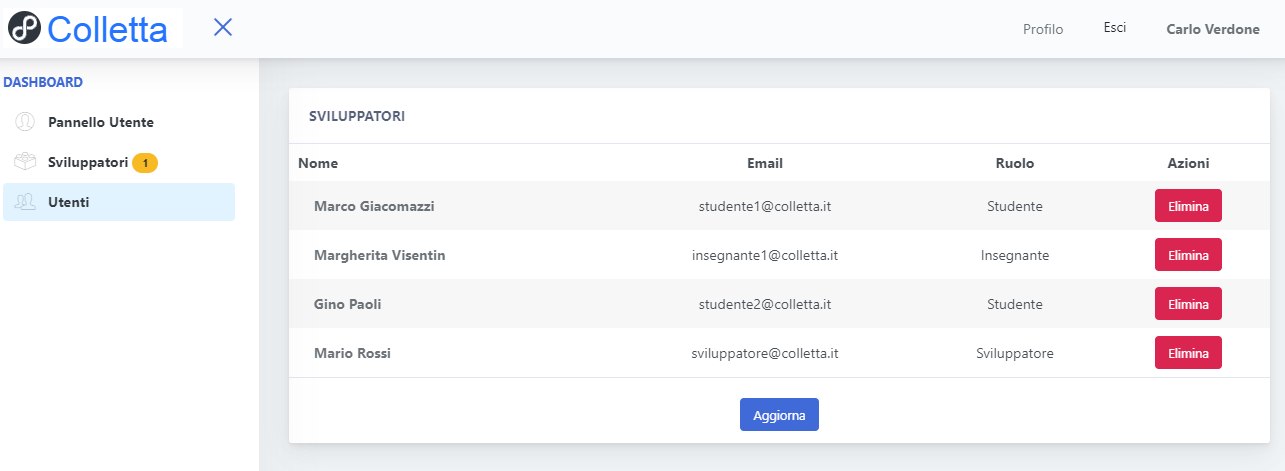
\includegraphics[width=17cm]{sez/img/amministratore/gestisciutenti.PNG}
				\caption{Gestione utenti}\label{fig:1}
			\end{figure}
		  In questa pagina l'amministratore può visualizzare gli utenti iscritti ed eventualmente eliminarli dal sistema. Per ogni utente sono presenti nome, email e ruolo (Insegnante, Sviluppatore o Allievi). Gli amministratori non figurano in questo elenco. 
		  
		  Cliccando su \textit{Elimina}, compare un alert per la conferma dell'eliminazione, cliccando su \textit{Si} l'utente viene eliminato, cliccando \textit{No} l'operazione viene annullata. Premendo su \textit{Aggiorna} la lista degli utenti viene aggiornata.
